% !TeX spellcheck = en_US
\documentclass[11pt]{article}

\usepackage[hmargin=3.1cm,vmargin=2.4cm]{geometry}
\usepackage{mathtools}
\usepackage[dvipsnames]{xcolor}
\usepackage{amssymb,dsfont,stmaryrd}
\usepackage{algorithm2e}
\usepackage{hyperref,cleveref}
\usepackage{graphicx}
\usepackage{booktabs}
\usepackage{subcaption}
\usepackage{enumitem}
\usepackage{titlesec}
\usepackage{tikz}

\usetikzlibrary{bayesnet,arrows,backgrounds}


\setlist{itemsep=0pt}

\hypersetup{
	colorlinks,
	urlcolor=NavyBlue
}

%%% Math macros %%%

\newcommand\RR{\mathbb{R}}
\newcommand\CC{\mathbb{C}}
\newcommand\ZZ{\mathbb{Z}}
\newcommand\NN{\mathbb{N}}
\newcommand\TT{\mathbb{T}}
\newcommand\PP{\mathbb{P}}
\newcommand\EE{\mathbb{E}}
\DeclarePairedDelimiter{\intinterv}{\llbracket}{\rrbracket}

\renewcommand{\epsilon}{\varepsilon}

\newcommand{\suchthat}{\mathrm{s.t.}}

\DeclareMathOperator*{\argmin}{\mathrm{argmin}}
\DeclareMathOperator*{\argmax}{\mathrm{argmax}}
\DeclareMathOperator{\diag}{\mathrm{diag}}
\DeclareMathOperator{\sgn}{\mathrm{sgn}}
\DeclareMathOperator{\trace}{\mathrm{Tr}}

\newcommand{\calM}{\mathcal{M}}
\newcommand{\calP}{\mathcal{P}}
\newcommand{\calN}{\mathcal{N}}
\newcommand{\calX}{\mathcal{X}}
\newcommand{\calL}{\mathcal{L}}
\newcommand{\calC}{\mathcal{C}}
\newcommand{\calD}{\mathcal{D}}

\newcommand{\bmmu}{\boldsymbol{\mu}}
\newcommand{\bmpsi}{\boldsymbol{\psi}}
\newcommand{\bmphi}{\boldsymbol{\phi}}

\newcommand{\bmX}{\boldsymbol{X}}


%%% Section titling setup %%%

\titleformat*{\section}{\LARGE\bfseries\sffamily}
\titleformat*{\subsection}{\Large\bfseries\sffamily}

\titleformat{\paragraph}[runin]{\sffamily\bfseries}{}{}{}[.]


%%% Document title %%%

\title{
	MVA -- Probabilistic Graphical Models\\
	{\color{NavyBlue}\sffamily Homework 3: Gibbs Sampling}
}

\author{
	Wilson \textsc{Jallet}\thanks{\url{wilson.jallet@polytechnique.org}}}


\begin{document}

\maketitle


\paragraph{Q1} This operation puts all the data on the same scale -- this is especially useful because the prior on $\beta$ assigns the same variance in each direction.


\paragraph{Q2} If we supposed that $\epsilon_i$ had a variance of $\sigma^2$, we could write $\epsilon_i = \sigma \epsilon'_i$ where $\epsilon'_i \sim \calN(0,1)$, and we'd have
\[
	y_i = \sgn(\beta^T x_i + \epsilon_i) =
	\sgn({\beta'}^T x_i + \epsilon'_i)
\]
where $\beta' = \beta/\sigma$.


\paragraph{Q3} We define the following graphical model:
\begin{itemize}
	\item observed features $x_i \in \RR^p$, $i\in\{1,\ldots,n\}$
	\item random variable $\beta\sim \calN(0, \tau I_p)$
	\item latent variables $z_i = \beta^Tx_i + \epsilon_i$, $\epsilon_i \sim \calN(0,1)$
	\item observed labels $y_i = \sgn(z_i) \in \{-1,1\}$
\end{itemize}

This model has the following representation:
\begin{figure}[h]
	\centering
	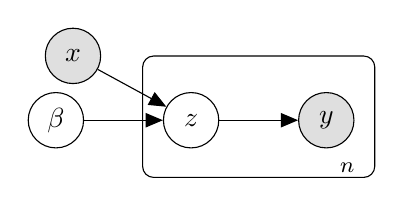
\begin{tikzpicture}
	\node[obs] (y) {$y$};%
	\node[latent,left=of y] (z) {$z$}; %
	\node[latent,left=of z] (beta) {$\beta$}; %
	% plate
	\plate [inner sep=.25cm,yshift=.2cm] {plate1} {(y)(z)} {$n$}; %
	% edges
	\edge {z} {y};
	\edge {beta} {z};
	
	\node[obs,above=of z,xshift=-1.5cm,yshift=-9mm] (x) {$x$};
	\edge {x} {z};
	\end{tikzpicture}
\end{figure}

We want the posterior distribution of $\beta$ given $y$. We will need the conditional posteriors to do Gibbs sampling.
Evidently,
\begin{align*}
	p(y_i|\beta)
	= \Phi(y_i\beta^Tx_i)  \\
	p(z_i | \beta)  \sim \calN(\beta^T x_i, 1)  \\
	p(y_i,z_i|\beta) = \mathds{1}_{\{y_iz_i > 0\}}
\end{align*}
By Bayes' theorem we have the posteriors
\begin{align*}
	p(\beta|z) \propto p(\beta)p(z|\beta)
	&\propto \exp\left(
		-\frac1{2\tau}\|\beta\|^2
		-\frac{1}{2}\sum_{i=1}^{n}(z_i - \beta^T x_i)^2
	\right)  \\
	&= \exp\left(
		-\frac1{2\tau}\|\beta\|^2
		-\frac{1}{2}\|z - X\beta\|^2
	\right)
\end{align*}
and
\begin{align*}
	p(z|\beta,y) \propto p(z|\beta)p(z,y|\beta)
	&\propto \exp\left(
	-\frac{1}{2}\|z - X\beta\|^2
	\right) \prod_{i=1}^{n} \mathds{1}_{\{y_iz_i > 0\}}
\end{align*}
where $X = (x_1|\ldots|x_n)^T \in \RR^{n \times p}$ is the design matrix. By identification $\beta|z \sim \calN(\mu, \Sigma)$ where
\[
	\Sigma^{-1} = \frac{1}{\tau}I_p + X^TX,
	\quad
	\mu = \Sigma X^Tz
\]
and $z|\beta,y \sim \mathrm{T}\calN(X\beta, I_n; \calP_y)$ where $\mathrm{T}\calN(\cdot; \calP_y)$ is the truncated Gaussian with support in the polytope $\calP_y = \{z\in\RR^n : z_i y_i > 0,\ i=1,\ldots,n\}$.


\end{document}
